\documentclass[sigconf,anonymous]{acmart}
\usepackage{booktabs} % For formal tables
\usepackage{graphicx}
%\usepackage{subfigure}
\usepackage{subfig}
\usepackage{xspace}
\usepackage{enumitem}
\usepackage{verbatim}
\usepackage{url}
\usepackage{hyperref}
\usepackage{algorithm}
\usepackage[noend]{algpseudocode}
\usepackage{amsmath}
\usepackage{multirow}
\usepackage{etoolbox}
\usepackage{gensymb}
\usepackage{mathtools}

\settopmatter{printacmref=false}
%%
%% end of the preamble, start of the body of the document source.
\begin{document}
\sloppy
%%
%% The "title" command has an optional parameter,
%% allowing the author to define a "short title" to be used in page headers.
%\title{On the Throughput Predictability in 60 GHz WLANs}
\title{Throughput Prediction on 60 GHz Devices for Latency Sensitive Applications}

%%
%% The "author" command and its associated commands are used to define
%% the authors and their affiliations.
%% Of note is the shared affiliation of the first two authors, and the
%% "authornote" and "authornotemark" commands
%% used to denote shared contribution to the research.
% \author{Ben Trovato}

% \renewcommand{\shortauthors}{Trovato and Tobin, et al.}
\fancyhead{}
\renewcommand\footnotetextcopyrightpermission[1]{}
%%
%% The abstract is a short summary of the work to be presented in the
%% article.
\begin{abstract}

In the near future, high quality VR and video streaming at 4K/8K resolutions will require Gigabit throughput to maintain a high user quality of experience (QoE). IEEE 802.11ad, which standardizes the 14 GHz of unlicensed spectrum around 60 GHz, is a prime candidate to fulfil these demands wirelessly. To maintain QoE, applications need to adapt to the ever changing network conditions and hence perform quality adaptation. One key component of quality adaptation is throughput prediction. At 60 GHz, due to the much higher frequency, the throughput can vary sharply due to blockage and mobility. Hence, the problem of predicting throughput becomes rather challenging.

In this paper, we show that there is a clear region in the
field-of-view (FoV) outside which 60 GHz does not work. We also show
that within this FoV, throughput may not always be stable as has been
previously claimed. Using neural networks, we predict the throughput
for the 60 GHz link at different timescales, from 10 ms (suitable for
VR) up to 2 s (suitable for ABR streaming). We show that we can 
accurately predict the throughput for various realistic scenarios
across different time scales.

\end{abstract}

%%
%% This command processes the author and affiliation and title
%% information and builds the first part of the formatted document.
\maketitle

\graphicspath{{figs/}}

\section{Introduction} % 1 page

Over the past few years consuming video content has become
tremendously popular. As of 2019, YouTube had 2 billion logged-in
monthly users~\cite{statista} and more than 73\% of adults in the US
watched videos on YouTube~\cite{pew-research}. More recently, there
have been an influx of novel types of multimedia content such as
360\degree~videos, volumetric videos, and VR gaming. Users also have
novel ways to consume such content, such as through a head mounted
display (HMD). 
% However, such content also has a higher demand in terms
% of the user's quality of experience (QoE). 
However, video streaming is
known to be challenging; the network conditions between the server and
the user inevitably have variations, which could cause a user watching
a 360\degree~video or playing a VR game to experience a long start up
time or periods of rebuffering/stalls. Such experiences can have
different consequences for different types of content. For example, a
user watching a video that keeps getting stalled may just stop
watching the video while a user playing a VR game might suffer from
motion sickness.

To deal with such issues, adaptive bitrate (ABR) streaming has become
one of the most popular techniques to stream multimedia
content. Consequently, a number of adaptive streaming standards have
been introduced over the years~\cite{stockhammer:mmsys2011,
  pantos-hls, adobe-hds, microsoft-ss}. ABR streaming monitors the
network conditions and adapts the content quality to minimize the
occurrences of such issues, which could drastically impact the user
QoE. One of the main components of adaptive bitrate streaming is the
estimation of network conditions. Traditionally, most ABR systems
calculate throughput estimates and choose a quality level based on the
download speeds of the past chunks and/or playback buffer
occupancy~\cite{sun:sigcomm2016, spiteri:infocom2016}. More recently,
the use of machine learning (ML) to select the most appropriate
quality level has gained significant popularity~\cite{mao:sigcomm2017,
  yan:nsdi2020} and ML-based ABR algorithms have been shown to
outperform traditional ones.

Due to the recent advancements in multimedia technology, video content
is getting richer with higher resolution and better quality. However,
this also means that applications that provide such content demand
much more bandwidth from the underlying network. For example, most
high quality VR setups today are tethered because today's wireless
networks are unable to provide the necessary capacity to support such
applications. However, with the advent of mmWave technologies like 5G
(for cellular networks) and 802.11ad (for indoor WLANs), these
applications can potentially go wireless. For example, the IEEE 802.11ad
wLAN standard~\cite{80211ad} governs the use of the 14 GHz of
unlicensed spectrum around 60 GHz. The standard supports 2 GHz wide
channel and provides PHY data rates of up to 6.7 Gbps which is ideal
to satisfy the needs for such applications.

However, due to their much higher frequency of operation, 60 GHz networks have vastly different propagation characteristics from sub-6 GHz networks. Due to the high attenuation loss at 60 GHz, directional communication is needed. This makes the wireless link highly susceptible to human blockage and mobility. Due to these challenges, a user watching a 360\degree~video or playing a VR game over a 60 GHz network can experience large periods of rebuffering/stalls due to intervals of low to no 60 GHz connectivity. For example, the user may be moving around or rotating in such a way so as to face completely away from the access point and thus self-block the link. Hence, even if 60 GHz wireless is used to enable these high resolution applications, it cannot be used as a standalone technology. One way to keep the rebuffering and stalls to a minimum while using 60 GHz is to use legacy sub-6 GHz WiFi, which does not suffer from these issues of blockage and mobility, as a backup.
 %This means that there will be a drop in content quality due to the use of slower sub-6 GHz ne% twork but will still lead to better user QoE than when there are stalls. 
These unique characteristics of the 60 GHz links make throughput prediction in 60 GHz WLANs a much more important and challenging problem than in legacy WLANs.

In this work, {for the first time}, we study the throughput predictability in 60 GHz wireless LANs using machine learning. In the past, throughput estimation/prediction has been studied in the context of sub-6 GHz wireless networks~\cite{khan:infocom2016,song:secon2017,kajita:wmnc2015} and mobile networks~\cite{liu:globecom2015}. However there has been no previous work, to our best knowledge, that has studied throughput prediction at mmWave frequencies such as 60 GHz. 

There are 2 main challenges we face to conduct this study. First, to
reliably train and test any machine learning model, a significant
amount of data is needed.~\cite{mao:sigcomm2017} used over 30 hours of
network traces, ~\cite{yan:nsdi2020} collected data for over a million
video streams, and~\cite{xu:conext2017} collected over 150 hours of
video playback data through user trials. Since 60 GHz WLANs are not
widely deployed (the first 802.11ad-enabled smartphones were only
launched in 2019), we cannot collect data from real networks, unlike
in ~\cite{mao:sigcomm2017,yan:nsdi2020}. Also, the only 2 phones that
support 802.11ad are not VR Ready and so we could not perform real VR
experiments with volunteers. Thus, we wanted a way to collect
traces in a controlled environment efficiently and in an automated way
while still considering the importance of performing realistic
mobility patterns. To meet these conflicting requirements, we mounted
the smartphone on a programmable 3-axis motion controller and slider
typically used by professional photographers. Using this setup, we
were able to collect more than 100 hours of traces while running
different applications and performing various controlled and random
mobility patterns. The second challenge is that, unlike previous
works, which make predictions only on coarse-grained timescales (in
the order of a few seconds) for ABR video streaming, we study prediction at
timescales as low as 10 ms (targeting VR applications). Hence, we need
ML models that strike the right balance between being accurate as well
as being lightweight enough to run on mobile devices within such short
timescales.

\if 0 With this study, we aim to answer the question: Can 60 GHz
throughput be predicted at various timescales and be used by latency
sensitive applications for quality adaptation? We use neural networks
to predict throughput using the past throughput data, 60 GHz link
information as well as data from the smartphone's motion and
orientation sensors. Our goal, in terms of the neural network model,
is to achieve high accuracy while making sure the model is lightweight
and hence can be run on hardware present on today's mobile devices. To
collect a large enough data set with realistic mobility patterns to
properly train and test our ML models, we mounted the smartphone on a
3-axis motion controller and slider typically used by professional
photographers. Using this setup we were able to collect more than 100
hours of traces while running different applications and performing
various controlled and random mobility patterns.  \fi Our
contributions and findings are summarized as follows:

\begin{itemize}
    \item ???
\end{itemize}

\section{Motivation} % 1 page

\subsection{Latency Sensitive Applications}

% Please add the following required packages to your document preamble:
% \usepackage{booktabs}
% \usepackage{multirow}
\begin{table*}[t]
\caption{Requirements of Latency Sensitive Applications}
\label{tab:apps}
\begin{tabular}{@{}cc|c|c|c@{}}
\toprule
                                      &    & Bandwidth      & Latency                         & QoE                                                                                                                      \\ \midrule
\multirow{2}{*}{Virtual Reality}                   & 4K & 300 Mbps       & \multirow{2}{*}{16 ms (60 fps)} & \multirow{2}{*}{\begin{tabular}[c]{@{}c@{}}Motion-to-photon latency \textless 20 ms, frame rate 60 fps\end{tabular}}    \\
                                      & 8K & 1.2 Gbps       &                                 &                                                                                                                          \\ \midrule
\multirow{2}{*}{360\degree~video streaming} & 4K & 50 Mbps        & \multirow{2}{*}{33 ms (30 fps)} & \multirow{2}{*}{\begin{tabular}[c]{@{}c@{}}Motion-to-photon latency \textless 20 ms, frame rate 30-60 fps\end{tabular}} \\
                                      & 8K & 200 Mbps       &                                 &                                                                                                                          \\ \midrule
Live streaming                        & 4K & Up to 1.8 Gbps & 33 ms (30 fps)                  & Frame rate 30-60 fps                                                                                                     \\ \bottomrule
\end{tabular}
\end{table*}
% Motivation
% Need throughput prediction to do adaptation
% to maintain QoE
% Table with BW, Latency, QoE requirements

Applications such as VR, 360\degree~video streaming, and live video
streaming need to maintain a certain latency in order to provide the
user with an acceptable quality of experience
(QoE). Table~\ref{tab:apps} lists the requirements for these
applications in terms of bandwidth, latency and QoE.

Network conditions between the server and the client will inevitably have some variations. Thus, for an application to maintain the required latency (and in turn QoE), it is necessary to adapt to these evolving network conditions. Most applications do this in the form of quality/bitrate adaptation.

To perform this adaptation, the server or client needs a way to detect the change in network capacity and react to it. In HTTP-DASH, the client estimates the available bandwidth and requests the next chunk based on that estimate~\cite{stockhammer:mmsys2011}. Most ABR clients use the download rates of the past ABR chunks to get this estimate~\cite{bentaleb:cst2019}.

Table~\ref{tab:apps} details the requirements of latency sensitive
applications in terms of the bandwidth, latency and QoE. As we can
see, there are applications like 8K VR and live video streaming which
require Gbps throughputs. Since the current generation of WiFi is not
capable of delivering those speeds, 60 GHz wireless is a prime
candidate to fulfil these needs. But, due to the nature of 60 GHz
wireless, throughput prediction becomes rather important as ABR
schemes would find it difficult to react to the sudden throughput
changes inherent at such a high frequency. Note that these throughput
changes also make the prediction of throughput at 60 GHz quite
challenging.\Comment{this paragraph doesn't seem to belong here?}

\subsection{802.11ad}
% Basic explanation of the standard

The 802.11ad standard defines 2 GHz wide channels (an order of magnitude wider compared to legacy WiFi), which enable Gbps data rates. The standard defines 12 MCSs for data frame transmission for the single-carrier (SC) PHY that is used by all commercial-off-the-shelf (COTS) devices, yielding data rates from 385-4620 Mbps. 

At the MAC layer, the main difference between the IEEE 802.11ad
standard compared to the standards governing legacy WiFi is the use of
directional communication. Directional communication is required due
to the much higher attenuation at the 60 GHz frequency band. To enable
directional communication, 802.11ad devices (both APs and clients)
perform Sector Level Sweeps (SLS) to train their transmit
sectors. During an SLS, each device transmits a Sector Sweep (SSW)
control message on each of its transmit sectors, while the other
device listens omnidirectionally. Once both sides have transmitted the
SSW message on all their transmit sectors, they exchange feedback
messages indicating to the other side which of their transmit sectors
resulted in the highest SNR. The standard does not define the
periodicity of the SLS. COTS devices typically perform an SLS every few
seconds. In addition, an SLS is triggered during data transmission in
case of a missing Block ACK after the number of MAC retries is
exceeded.


\section{Experimental Methodology} % 1 page

In this section, we describe the devices we use, the measurement methodology, and the machine learning models.

\subsection{Devices}

We use a Netgear Nighthawk X10 Smart WiFi router~\cite{netgear-x10} and an ASUS ROG Phone II~\cite{rog-phone-2} for all our measurements. The Netgear router is one of the two 802.11ad-compliant routers on the market. It has a 10-Gigabit SFP+ Ethernet port, which we use to connect to a powerful desktop acting as the server in our experiments. The ASUS ROG Phone II is the second widely available smartphone with an 802.11ad chipset after its pre-decessor, the ASUS ROG Phone~\cite{rog-phone}. It houses an octa-core Snapdragon 855 Plus processor with a maximum CPU frequency of 2.96 GHz. It has a 6000 mAh battery, an 8 GB RAM and runs the Android OS 10. Both devices support all 12 802.11ad SC MCSs, yielding theoretical data rates up to 4.6 Gbps. However, similar to previous studies using laptops as clients instead of smartphones~\cite{sur:mobicom2017,saha:secon2018,baig:mobicom2019,saha:mobicom2019}, we found that the maximum throughput is limited to 2.3 Gbps when the phone is placed right in front of the AP and to 1.65 Gbps in most practical scenarios.

%is used as our client device. It is . It consists of an 8-element phased antenna array. Similar to the Netgear router, it supports data rates up to 4.6 Gbps. However, we found that performance is limited to $\sim$2.3 Gbps when the phone is placed right in front of the router and under most practical scenarios, it is limited to $\sim$1.6 Gbps.



%The Netgear router uses the 802.11ad QCA9008-SBD1 module with the QCA9500 chipset from Qualcomm, supporting single-carrier data rates up to 4.6 Gbps. It contains a 32-element phased antenna array %hich is connected to the chipset via an MHF4 cable. It has a 10-Gigabit SFP+ Ethernet port which we use to connect to a powerful desktop which acts as the server in our experiments.



\subsection{Methodology}

For all our experiments, we keep the phone in a Google
Cardboard~\cite{cardboard} headset at a distance of 4 m from the
AP. We used nuttcp~\cite{nuttcp} to generate TCP traffic and log
throughput every 10 ms. We developed an Android application that runs
on the phone and uses the Android Sensor API~\cite{android-sensor} to
log information from the
$\tt{TYPE\_ROTATION\_VECTOR}$/$\tt{TYPE\_GAME\_ROTATION\_VECTOR}$. These
sensors report the angle (in radians, which we convert to degrees) that the
phone has moved in the azimuth, pitch, or roll directions. We also log
data from the accelerometer ($\tt{TYPE\_ACCELEROMETER}$) sensor, which
gives the acceleration of the phone (in m/s$^2$) in the x-, y-, and
z-axis. Data from both the sensors are logged every 10 ms.

In addition to the above information, we also log 60 GHz link information reported by the $\tt{wil6210}$ driver on the phone. This includes the MCS used by the AP-phone link for data transmission, link quality estimators (SQI, RSSI), and the phone's and AP's beamforming sectors. This information is logged every 20 ms.

For the experiments involving mobility, we use a Cinetics Lynx 3-Axis Slider~\cite{cinetics-lynx} and attach the Google Cardboard headset to it. This motion controller and slider enables us to perform full 360\degree~rotation in the azimuth and pitch directions at a speed of up to nearly 50\degree/s. The slider allows us to move the phone in a translation motion of up to 1 m. The Lynx setup has support for the Dragonframe software~\cite{dragonframe}, which we use to program custom mobility patterns and automate the trace collection process. Fig.~\ref{fig:setup} shows this setup and the 3 axes of motion.

%\Comment{Put a figure and define pitch, azimuth and slide}

\begin{figure}[t]
    \centering
    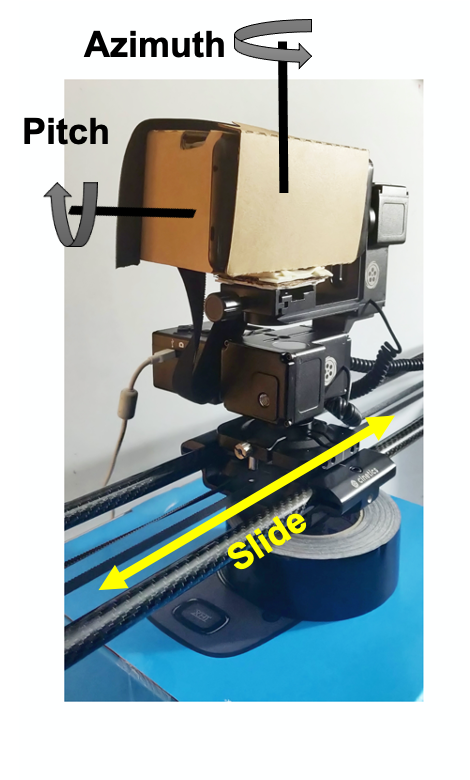
\includegraphics[width=0.2\textwidth]{setup.png}
    \caption{Mobility Experiments Setup}
    \label{fig:setup}
\end{figure}

\subsection{Trace Processing}

Applications have a diverse requirement on the timescale of throughput prediction. VR applications for example, need to predict the throughput in the window of the next tens of milliseconds. On the other end of the spectrum, video streaming applications usually fetch video chunks of several seconds in length and therefore need to predict the average throughput in the window of the next few seconds. We are interested in the throughput predictability over 802.11ad at all these timescales, and hence we experiment with representative timescales of 10 ms, 20 ms, 40 ms, 100 ms, 200 ms, 400 ms, 1000 ms, and 2000 ms.

To convert the throughput traces, which log throughput samples every 10 ms, to other timescales, we combine every few consecutive samples. For example, to obtain 20ms traces, every 2 adjacent data points are combined. Within each window, the throughput is averaged to produce the mean throughput in the window. For all other features, we consider the last data point in the window. This is because those features (e.g., MCS, Transmit sector) consist of categorical values, and are not meaningful when averaged. In addition, during prediction the last value in the window can more accurately reflect the up-to-date state of the feature.

To make a fair comparison across different timescales, we always use the same amount of data for training as well as testing: the first 15,000 data points for training, and the following 3,000 for testing.

We collected a total of XX hours of traces consisting of XX samples.

\subsection{Machine Learning}
\label{subsection: Machine Learning}

We use neural networks to make throughput predictions. We experimented with 3 neural networks. For each network, we experimented with various configurations and picked the one that performs the best.

\textbf{BP8}: a shallow fully-connected neural network with 3 hidden layers, each of 40 neurons. It takes as input the actual throughput in the past 8 windows, pose information in the past window, and link layer information in the past 1 window.

\textbf{RNN8}: a recurrent neural network with 3 hidden layers, each with 20 neurons. It takes as input the actual throughput, pose information, and link layer information in the past 8 windows.

\textbf{RNN20}: same as BP8, but takes information in the past 20 windows as input.
\Comment{Do we need to explain why BP8 takes historic values of only throughput, but RNN takes historic values of all features?}

Specifically, the pose information consists of azimuth and pitch. The link layer information consists of MCS, transmit beamforming sector, link status, SQI, and RSSI.

% The neural network takes as input:
% \begin{enumerate}
%     \item The actual throughput in the past N windows $T_{t-N}, T_{t-N+1}, ..., T_{t-1}$,
%     \item Pose information in the past 1 window (azimuth, pitch),
%     \item 60 GHz link layer information in the past 1 window (MCS, transmit beamforming sector, link status, SQI, RSSI)
% \end{enumerate}

The neural network outputs the probability distribution of the throughput in the current window $T_{t}$. The probability distribution $P_{1}$, $P_{2}$, $P_{3}$, ..., $P_{21}$ is over 21 bins of throughput in Mbps: $B_{1}=[0,50)$, $B_{2}=[50, 150)$, $B_{3}=[150, 250)$, ..., $B_{21}=[1950, 2000]$. We calculate the expected throughput based on the probability distribution as the prediction output:

\begin{equation}
Throughput = 0 \times P_{1} + \sum_{i=2}^{20} median(B_{i}) \times P_{i} + 2000 \times P_{21}
\end{equation}

% The network is a fully-connected neural network. We tested various network architectures by varying the number of hidden layers and neurons, and picked the best model to be with 3 hidden layers, each with 40 neurons.

\subsection{Metrics}
We evaluate the performance of the throughput prediction model in terms of 3 metrics:

\begin{enumerate}
    \item The root mean squared error (RMSE) between the prediction and the actual throughput.
    \item The absolute relative error of the prediction at 95\% percentile. (ARE95)
    \item The percentage of predictions with absolute relative error below 10\%. (PARE10)
\end{enumerate}

To understand which input features are the most useful for a high prediction accuracy, we also run a feature selection algorithm which ranks the importance of the features.

\section{Results} % 4 pages
\label{section: Results}

In this section, we present the results using our neural network model moving from simpler to more realistic but also more complex scenarios. We consider four types of scenarios: (i) static scenarios, where the phone is fixed at a given azimuth and pitch at a distance of 4 m in front of the AP, (ii) controlled mobility scenarios, where the phone moves along one dimension (azimuth, pitch, or slide) at a given speed keeping the other two dimensions constant, (iii) random mobility scenarios, where the phone simultaneously moves along all three dimensions at different speeds, and (v) real applications scenarios, where we use 2 real application traces -- VR and ABR video streaming -- instead of backlogged TCP traffic generate by nuttcp, under random mobility. 

\subsection{Impact of Field of View (FoV)}

We first analyze the impact of the phone staying within the AP's field of view (FoV). The phone faces the AP from a distance of 4 meters, and we rotate the phone to change its azimuth with respect to the AP. Fig.~\ref{} plots the throughput at the phone when the phone is rotated to the different angles. Our experiments show that when the azimuth is within [-75\degree, 75\degree], the average throughput is always $\sim$1.5 - 1.6 Gbps. Once the azimuth moves outside this region, the throughput quickly drops to 0, meaning that the AP fails to find a stable transmit sector at this angle as the phone's omnidirectional receive beam is out of the FoV of the AP. This agrees with the findings by the authors of~\cite{wei:mobicom2017}. Following this, in the rest of the paper we only focus on predicting throughput when the phone is within the AP's FoV.

We also noticed that even within the FoV, the instantaneous throughput is not always stable, but varies between 1.2 Gbps and 1.6 Gbps, which is caused by the 802.11ad MAC layer mechanisms such as the beacons sent out by the AP every 100 ms or beamforming between the phone and the AP. Hence, these variations are unavoidable when using an 802.11ad link.

\subsection{Static Conditions}

Next, we explore the throughput predictability when the phone is static and is within the AP's FoV. The purpose is to understand how well we can predict throughput changes caused by channel variations only.

We collected 5 static traces listed in Table \ref{tab: Static Traces Collected} where we place the phone at various azimuth and pitch angles with respect to the AP. We trained and evaluated a separate model on each trace. The models are described in \S\ref{subsection: Machine Learning}. %In our experiments, the model takes the past 8 windows' throughput as input.

\begin{table}[h!]
\caption{Static Traces Collected}
\label{tab: Static Traces Collected}
\begin{tabular}{c|c c c c}
\toprule
Trace \# & Azimuth & Pitch & Length & Throughput (Mbps) \\
\midrule
Static 1 & 0\degree & 0\degree & 10hr & 1588 $\pm$ 209 \\
Static 2 & 30\degree & 0\degree & 10hr & 1575 $\pm$ 238 \\
Static 3 & 60\degree & 0\degree & 10hr & 1568 $\pm$ 307 \\
Static 4 & 0\degree & 40\degree & 10hr & 1566 $\pm$ 238 \\
Static 5 & 0\degree & -40\degree & 10hr & 1585 $\pm$ 203 \\
\bottomrule
\end{tabular}
\end{table}

\subsubsection{Model Performance}
\label{subsubsection: Model Performance}

We train 3 models (BP8, RNN8, RNN20) for each trace at each resolution, and evaluate the models using the metrics described in \S \ref{section: Results}. The results shown in Figure~\ref{Static Conditions} are averaged over the 5 traces detailed in Table~\ref{tab: Static Traces Collected}.

\begin{figure}[h]
\centering
\subfloat[Mean squared error]{
    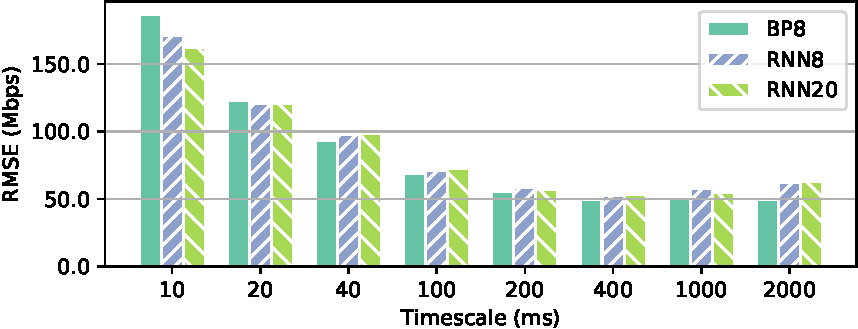
\includegraphics[width=0.45\textwidth]{rmse_barplot.pdf}
    \label{subfig:static_mse}
}
\hfill
\subfloat[Absolute relative error at 95\% percentile]{
    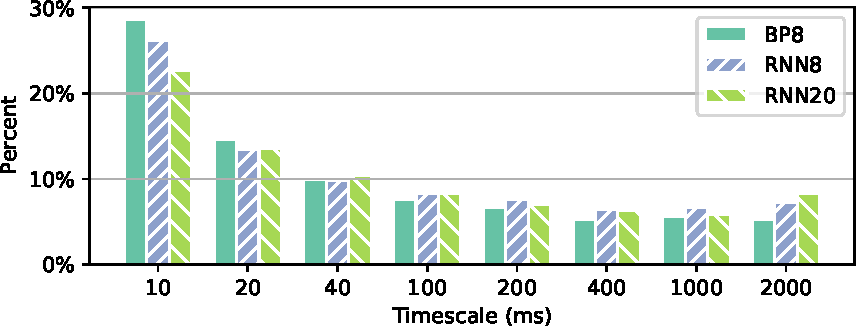
\includegraphics[width=0.45\textwidth]{abs_rel_err_95_barplot.pdf}
    \label{subfig:static_abs_rel_err_95}
}
\hfill
\subfloat[Percent of predictions with absolute relative error below 10\%]{
    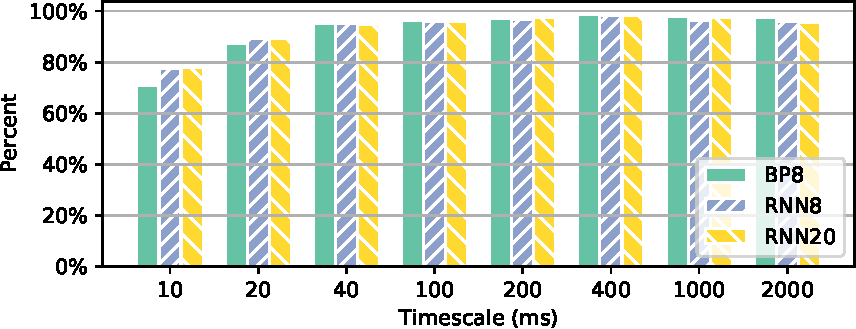
\includegraphics[width=0.45\textwidth]{perc_error_10perc_barplot.pdf}
    \label{subfig:static_perc_error_10perc}
}
\caption{Model Performance for Static Traces}
\label{Static Conditions}
\end{figure}

Overall, Fig.~\ref{Static Conditions} shows that as the timescale goes from 10 ms to 200 ms the performance of all 3 models improves significantly for all 3 metrics. At timescales larger than 200 ms, the increase in model performance becomes marginal. This expectedly shows that predicting throughput at shorter time scales is more challenging due to the much higher fluctuations in throughput caused by the 802.11ad MAC. As the timescale increases, the variations get averaged out and hence the models show better performance.
%It is worth mentioning as timescales gets larger than 400ms, the increase in model performance becomes marginal. For traces \#1 and \#4, we even noticed that there is a sweet spot around 400ms where the model performs the best.

However, even in the worst case, at the 10 ms timescale, the RMSE is between 162 and 187 Mbps for the different models (Fig. \ref{subfig:static_mse}). Also, Figs.~\ref{subfig:static_abs_rel_err_95} and~\ref{subfig:static_perc_error_10perc} show that for the RNN20 model (the best performing model at 10 ms), 95\% of the errors have absolute relative error less than 23\% and nearly 78\% of the errors have absolute relative error less than 10\% respectively. Hence, depending on the application, it may still be possible to tolerate this level of error. At timescales 40 ms or larger, the RMSE drops to less than 100 Mbps for all 3 models while ARE95 becomes less than 10\% and PARE10 shows that more than 95\% of the predictions had less than 10\% error. Thus, all models show a sharp increase in performance from the 10 ms timescale and are overall highly accurate.

Interestingly, for the finer timescales of 10 ms and 20 ms the RNN models, especially the RNN20, outperform the BP8 model. At the larger timescales the performance gap becomes smaller with the BP8 model becoming the more accurate one.
%At the 2 s timescale, the models predict throughput with RMSE of 49.5 to 63.1 Mbps.

% \textbf{ARE95.} Figure \ref{subfig:static_abs_rel_err_95} shows that the models predict throughput with 22.6\%-28.7\% absolute relative error at the 95th percentile from the 10ms timescale, to 5.3\%-8.3\% at 2s timescale.

% \textbf{PARE10.} From Figure \ref{subfig:static_perc_error_10perc} it can be seen that, at the 10ms timescale, 70.9\%-78.0\% of the time our models make predictions with absolute relative error below 10\% . As the timescale increases to 2s, 95.4\%-97.6\% of the time the models make predictions with less than 10\% error.

To understand how the model performs for each trace, we picked the best model for each trace at each timescale, and calculated the RMSE. The results are shown in Figure \ref{figure: RMSE for Static Traces}.

\begin{figure}[h]
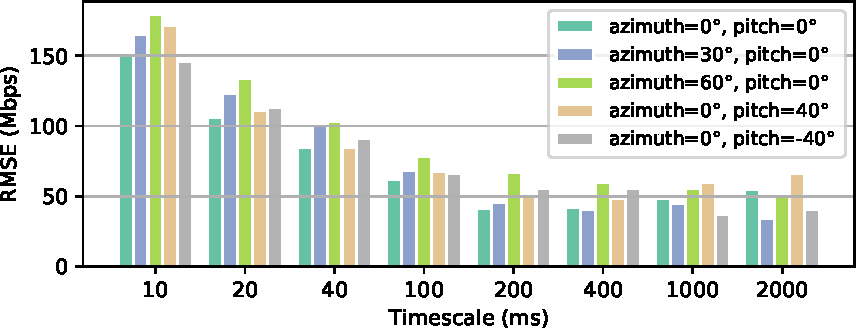
\includegraphics[width=0.45\textwidth]{figs/rmse_along_angle.pdf}
\caption{RMSE for Static Traces}
\label{figure: RMSE for Static Traces}
\end{figure}

\subsubsection{Feature Selection}
As mentioned in \S\ref{subsection: Machine Learning}, the inputs to the neural network model consist of 1) The actual throughput in the past 8 windows, 2) The pose information in the past window, and 3) The link-layer states in the past window. To understand which of these features are more useful in the prediction, we perform a feature selection algorithm, described in Algorithm \ref{algorithm: Feature Selection}.

\algnewcommand\algorithmicforeach{\textbf{for each}}
\algdef{S}[FOR]{ForEach}[1]{\algorithmicforeach\ #1\ \algorithmicdo}
\begin{algorithm}
\caption{Feature Selection}
\label{algorithm: Feature Selection}
\begin{algorithmic}[1]
\State $F\gets$Set of all features
\While{$size(F) > 1$}
    \State $featureToRemove \gets nil$
    \State $maxMse \gets 0$
    \ForEach {$f \in F $}
        \State $F' \gets F-f$ \Comment{Remove 1 feature}
        \State $model \gets train(F')$ \Comment{Train on remaining features}
        \State $mse \gets eval(model)$
        \If {$mse > maxMse$}
            \State $maxMse \gets mse$
            \State $featureToRemove \gets f$
        \EndIf
    \EndFor
    \State $F \gets F-featureToRemove$ \Comment{Remove the least useful f}
\EndWhile
\end{algorithmic}
\end{algorithm}

We start with all $N$ features. For each of the feature, we temporarily remove it from the input, and train a model using the remaining $N-1$ features. This procedure identifies the least useful feature among $N$ features, and we permanently remove this feature from the input. Then, we iterative perform the same procedure on the rest $N-1$ features, until all features have been removed. Effectively, this algorithm ranks the features by usefulness. The result of our experiments is shown in Table \ref{tab: Static Feature Selection}.

\begin{table}[h]
\caption{Features Selection for Static Traces}
\label{tab: Static Feature Selection}
\begin{tabular}{c c|c c|c c}
\toprule
\multicolumn{2}{c|}{10ms} & \multicolumn{2}{c|}{100ms} & \multicolumn{2}{c}{2000ms} \\
Removed & RMSE & Removed & RMSE & Removed & RMSE \\
\midrule
- & 186.87 & - & 69.39 & - & 49.45 \\
Azimuth & 171.72 & Azimuth & 68.45 & Tx Sector & 48.80 \\
Pitch & 167.53 & Tx Sector & 67.28 & RSSI & 48.47 \\
SQI & 166.52 & RSSI & 66.76 & Azimuth & 48.78 \\
RSSI & 166.70 & Link Status & 66.85 & Link Status & 48.59 \\
Tx Sector & 166.30 & Pitch & 66.25 & Pitch & 48.85 \\
Link Status & 166.63 & SQI & 67.47 & SQI & 49.15 \\
MCS & 167.99 & MCS & 69.91 & Throughput & 51.51 \\
\bottomrule
\end{tabular}
\end{table}
\Comment{As the features get removed, RMSE first goes down and then goes up. Does this cause confusion?}


\subsection{Mobile Conditions}

Then, we investigate the impact of mobility on throughput predictability. We mount the phone on a rotor which rotate along the azimuth and pitch axis, and collected the traces listed in Table \ref{tab: Mobile Traces Collected}. We collected 5 traces with controlled mobility, by programming the rotor to rotate back and forth between two coordinates at a given speed. We also collected a trace with random mobility, where the rotor was programmed to move along random waypoints at random speeds. All traces are 10 hours long.

\begin{table}[h!]
\caption{Mobile Traces Collected}
\label{tab: Mobile Traces Collected}
\begin{tabular}{c|c c c c c}
\toprule
Trace \# & Azimuth & Pitch & Speed & Length & Mean \\
\midrule
Controlled 1 & [-60\degree,60\degree] & [0\degree,0\degree] & 45\degree/s & 10hr & 1479.31Mbps \\
Controlled 2 & [-60\degree,60\degree] & [0\degree,0\degree] & 40\degree/s & 10hr & 1471.11Mbps \\
Controlled 3 & [-60\degree,60\degree] & [0\degree,0\degree] & 10\degree/s & 10hr & 1568.30Mbps \\
Controlled 4 & [0\degree, 0\degree] & [-40\degree,40\degree] & 12\degree/s & 10hr & 1560.19Mbps \\
Controlled 5 & [0\degree, 0\degree] & [-40\degree,40\degree] & 6\degree/s & 10hr & 1567.94Mbps \\
Random 1 & [-60\degree,60\degree] & [-40\degree,40\degree] & - & 10hr & 1585.88Mbps \\
\bottomrule
\end{tabular}
\end{table}

\subsubsection{Model Performance}
We follow the same methodology as in Section \S\ref{subsubsection: Model Performance} to train 3 models (BP8, RNN8, RNN20) for each trace at each resolution.

\subsection{Applications}

To further understand the throughput predictability, we collected traces using 2 real applications, VR and ABR. These two application have different requirements on the timescale of throughput prediction. The results are shown in Table \ref{tab: Model Performance for Real Applications}.

\begin{table}[h!]
\caption{Model Performance for Real Applications}
\label{tab: Model Performance for Real Applications}
\begin{tabular}{c|c c c|c c c}
\toprule
 & \multicolumn{3}{c|}{VR} & \multicolumn{3}{c}{ABR}\\
 & BP8 & RNN8 & RNN20 & BP8 & RNN8 & RNN20 \\
\midrule
RMSE & 156.78 & 163.65 & 163.66 & 114.54 & 115.77 & 113.87 \\
ARE95 & 29.08\% & 28.82\% & 27.92\% & 18.15\% & 17.72\% & 17.58\% \\
PARE10 & 72.79\% & 70.52\% & 69.24\% & 86.93\% & 86.10\% & 87.03\% \\
\bottomrule
\end{tabular}
\end{table}

\section{Related Work} % 1/2-1 column

% Throughput prediction
There have been a few works in the past that have studied throughput prediction. However most of the past works~\cite{mirza:sigmetrics2007, bui:ewc2014, liu:globecom2015} did not look at using it for latency sensitive applications which require throughput prediction at fine grained time scales.~\cite{sun:sigcomm2016} is one of the works which predicts throughput for video bitrate selection using a data-driven approach. However, they predict throughput for an epoch of 6 seconds whereas in this work we make predictions for a timescale of up to 2 seconds.~\cite{liu:atc2020} performs throughput estimation at a finer grained resolution to estimate the available bandwidth for each user as well as the total available bandwidth from the AP's perspective. To enable this, the authors of~\cite{liu:atc2020} needed to modify the AP's firmware. In our work however the prediction is done on the client side hence we don't need to perform any modifications on the AP.~\cite{liu:globecom2015} performed a study of various throughput prediction algorithms for mobile networks and found that all of them have the highest accuracy when predicting at a timescale of 100-300 seconds which is again too large of a timescale when considering the type of applications we look at in this work.

% mmWave
\cite{wei:mobicom2017,zhou:infocom2018} are a couple of the works which utlize 60 GHz wireless to enable applications such as VR, AR, and Miracast.~\cite{wei:mobicom2017} proposes the idea of having multiple APs and as the client device moves, it can keep switching to a different AP that works best for that position. This work showed that as the client moves out of the AP's FoV, the client's performance drops drastically and often loses connectivity. We also have a similar finding in this work. However, they did not look at the time-varying nature of throughput that we observed even when the phone is within the AP's FoV.~\cite{zhou:infocom2018} found that typical VR/Miracast motion can be rather unpredictable and hence lead to large and sudden drops in signal quality. Thus, they did not try to predict the throughput and instead devised a way to reduce the search space for 60 GHz beamforming.
%In terms of mmWave

\section{Conclusion}



%%
%% The acknowledgments section is defined using the "acks" environment
%% (and NOT an unnumbered section). This ensures the proper
%% identification of the section in the article metadata, and the
%% consistent spelling of the heading.
\begin{acks}
To Robert, for the bagels and explaining CMYK and color spaces.
\end{acks}

%%
%% The next two lines define the bibliography style to be used, and
%% the bibliography file.
\bibliographystyle{ACM-Reference-Format}
\bibliography{references}

%%
%% If your work has an appendix, this is the place to put it.
% \appendix

% \section{Research Methods}

% \subsection{Part One}

\end{document}
\endinput
%%
